%%%%%%%%%%%%%%%%%%%%%%%%%%%%%%
% Dataset 
%%%%%%%%%%%%%%%%%%%%%%%%%%%%%%
\section{Dataset}
All models are trained on a newly created dataset of dresses from Zalando, one of the most popular online fashion retailers in Europe \citep[p.1]{freno2017practical}. The initial dataset consists of article information and image URLs of all publicly available dresses listed on the website "zalando.de" at the time of creation in March 2024. As a first pre-processing step, all articles that do not offer a standardized and centered packshot image of the dress are removed. Afterwards, all images are downloaded, squared in 1024x1024 resolution, and centered. Additionally, the article information is subset to attributes that offer good data completeness and non-noisy labels. The subset consists of the attributes "brand", "price", "category", "fabric", "fit", "neckline", "pattern", "collar", "length", "shape" and "sleeve length". These attributes are cleaned such that similar but small categories are grouped and categories with very few samples are recoded as missing to reduce the dimensionality of each attribute. Since there is no standardized color attribute, the color of each dress is obtained using a pre-trained CLIP model \citep[p.2]{radford2021learning} and a fixed list of 14 colors. The final dataset consists of 14,060 images with the corresponding article information from 643 unique brands. A random sample of images from the dataset can be seen in figure \ref{fig:random_samples}.

\begin{figure}[ht]
    \centering
    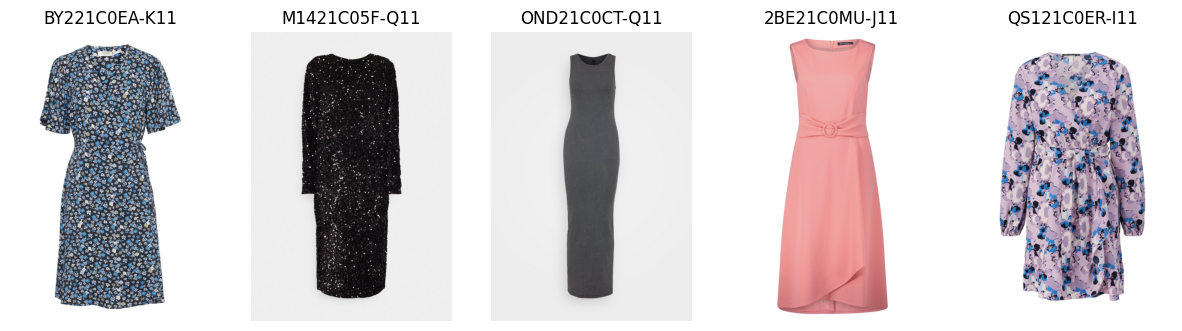
\includegraphics[width=1\linewidth]{Thesis/Dataset/random_sample.png}
    \caption{Random samples from the dataset}
    \label{fig:random_samples}
\end{figure}